\documentclass{article}

% Submission: default (main track, double-blind, with line numbers).
% After acceptance, replace with: \usepackage[main, final]{neurips_2026}
\PassOptionsToPackage{numbers, sort&compress}{natbib}
\usepackage[preprint]{neurips_2026}

\usepackage[utf8]{inputenc}
\usepackage[T1]{fontenc}
\usepackage{amsmath,amssymb,amsfonts}
\usepackage{graphicx}
\usepackage{booktabs}
\usepackage{hyperref}
\usepackage{url}
\usepackage{microtype}
\usepackage{xcolor}
\usepackage{subcaption}
\usepackage{multirow}
\usepackage{tikz}
\usetikzlibrary{positioning, arrows.meta, calc}
\usepackage{float}
\usepackage{placeins}
\usepackage{pgfplots}
\pgfplotsset{compat=1.18}
\usepgfplotslibrary{groupplots}

\graphicspath{{figures/}}

\newcommand{\todo}[1]{{\color{red}\textbf{[TODO: #1]}}}

\title{Tunable Non-linear Manifold ROMs for Elliptic and Parabolic
       PDEs via Matrix-Free Galerkin Projection}

\author{%
  Tahmid Awal, Cen-Jhih Li, Aditya Bhaskara, Hari Sundar \\
  Tufts University, University of Utah \\
  % \texttt{tahmid.awal@tufts.edu, }
}

\begin{document}
\maketitle

% =====================================================================
\begin{abstract}

Neural operators such as Fourier Neural Operators
\citep{Li2020FNO} and DeepONets \citep{Lu2021DeepONet} deliver one
(accuracy, speed) point per trained model and offer no way to tune
either at deployment. We present a non-linear manifold reduced order
model (NM-ROM) for elliptic and parabolic PDEs that exposes a
continuous accuracy/speed Pareto frontier from a single trained
decoder, controlled at inference time by three solver-side knobs: the
Gauss--Newton iteration cap, the Gauss--Newton tolerance, and the
empirical-quadrature (EQ) sample count. The framework combines a
matrix-free Galerkin projection of the discrete PDE residual onto a
learned manifold, evaluated through JAX
forward- and reverse-mode autodiff \citep{Bradbury2018JAX}; NNLS-based
\citep{LawsonHanson1974NNLS} EQ hyper-reduction
\citep{Hernandez2017EQ,YanoPatera2019LPEQ} that decouples residual cost
from mesh size; exact boundary condition enforcement by a binary
decoder mask; and a decoder architecture --- a Vision Transformer
encoder \citep{Dosovitskiy2021ViT,Vaswani2017Attention} feeding a
LinearCPDecoder \citep{KoldaBader2009CP} (linear skip + shallow MLP +
canonical-polyadic spatial head) --- that we identified by sweeping
decoder families against three constraints: cold-start latent
Gauss--Newton convergence, EQ compatibility, and sub-cubic parameter
scaling in mesh side. Across Poisson and Heat in 2D and 3D at multiple
resolutions, the trained-once Pareto frontier matches or beats FNO,
DeepONet, and the SMA-NM-ROM baseline of \citet{KimChoi2022NMROM} on
accuracy in most cells and is strictly faster than full-order
conjugate gradient \citep{HestenesStiefel1952CG}, reaching up to
$324\times$ wall-clock speedup.

\end{abstract}

% =====================================================================
\section{Introduction}
\label{sec:intro}

Neural operators for partial differential equations (PDEs)
\citep{Li2020FNO,Lu2021DeepONet,Kovachki2023NeuralOperator,Li2024PINO,BoulleTownsend2024} have
become a strong empirical baseline, but each trained model produces a
single fixed (accuracy, wall-clock) operating point: there is no
deployment-time knob a practitioner can turn to spend more compute for
more accuracy, or vice versa. Classical Full Order Methods (FOMs)
\citep{Hughes2000FEM} solved with conjugate gradient
\citep{HestenesStiefel1952CG} expose this knob through their iteration
tolerance, but at a wall-clock cost that is uncompetitive with neural
operators on the resolutions of interest.

Two families of methods sit on either side of this gap. Neural
operators and PDE foundation models
\citep{HerdePoseidon2024,McCabeMPP2024,HaoDPOT2024,Chen2024UnsupervisedNO} deliver fast
amortised inference but fix the accuracy/speed point at training time,
so the only way to recover a different point is to retrain. Reduced order
models (ROMs) address the same problem from the opposite direction: linear                       
projection-based ROMs \citep{BennerGugercinWillcox2015,Sirovich1987POD}                   
inherit the FOM's guarantees but hit the Kolmogorov $n$-width barrier                     
on advection-dominated regimes \citep{CohenDeVore2015}, and non-linear                    
manifold ROMs (NM-ROMs) \citep{LeeCarlberg2020,KimChoi2022NMROM} lift                     
this barrier with a learned manifold but have so far been demonstrated                    
mainly on 1D advection-dominated benchmarks rather than head-to-head                      
against neural operators on standard 2D/3D elliptic and parabolic                         
problems at production resolutions. The key open question is thus, is there a                        
single trained NM-ROM can match neural-operator accuracy, beat                            
classical CG in wall-clock at production mesh sizes, and expose a                         
deployment-time accuracy/speed tradeoff that neither alternative offers?                                                                                                                  

This paper answers that question affirmatively for 2D and 3D Poisson
and heat equations. We present an NM-ROM framework whose distinguishing                 
property is a \emph{deployment-time accuracy/speed Pareto curve traced                  
by a single trained model}: at inference, three solver-side knobs ---                   
the Gauss-Newton iteration cap, the Gauss-Newton early-exit tolerance,                  
and the Empirical Quadrature sample count --- continuously trade                        
accuracy for speedup. The supporting machinery is a masked decoder                     
that enforces Dirichlet boundary conditions exactly, a latent                           
Gauss-Newton solver \citep{NocedalWright2006} for elliptic problems and                   
backward-Euler latent solver for parabolic problems, NNLS-based                         
Empirical Quadrature hyper-reduction                                                    \citep{Hernandez2017EQ,YanoPatera2019LPEQ,LawsonHanson1974NNLS} that                    
decouples residual cost from mesh size, and a matrix-free JAX                           
implementation \citep{Bradbury2018JAX} of every projected operator.

\paragraph{Contributions.}
\begin{enumerate}
\item \textbf{A tunable NM-ROM with a deployment-time accuracy/speed
      Pareto curve from a single trained model.} Our primary
      contribution: at inference, three solver-side knobs (GN cap,
      GN tolerance, EQ samples) continuously trade rel-$L^2$ for
      wall-clock. Neural operators
      deliver one fixed
      (accuracy, speed) point per training run; a single trained
      NM-ROM exposes a continuous frontier covering 12$\times$ to
      191$\times$ speedup over CG at comparable accuracy across our
      2D/3D Poisson and heat benchmarks.
\item \textbf{Architectural choices that make this Pareto curve
      achievable.} We identify the three constraints a decoder must
      satisfy --- cold-start Gauss-Newton convergence, EQ
      compatibility, and sub-cubic parameter scaling in mesh side ---
      and show that the smallest architecture meeting all three is
      a ViT encoder 
      feeding a LinearCPDecoder
      \citep{KoldaBader2009CP}: linear skip + shallow MLP +
      rank-$R$ canonical-polyadic spatial head.
\item \textbf{A matrix-free JAX implementation that makes the
      framework practical.} Exact Dirichlet enforcement by decoder
      masking, NNLS-based Empirical Quadrature
      \citep{Hernandez2017EQ,YanoPatera2019LPEQ}, and JAX-autodiff
      \citep{Bradbury2018JAX} matrix-free evaluation of every
      projected operator together turn the framework into a single
      kernel that runs faster than the full-order CG solve and the neural-operator
      baselines.
\end{enumerate}


% =====================================================================
\section{Related Work}
\label{sec:related}

\paragraph{Linear and non-linear manifold ROMs.}
Linear projection-based ROMs
\citep{BennerGugercinWillcox2015,Sirovich1987POD,Berkooz1993,QuarteroniManzoniNegri2015,HesthavenRozzaStamm2016}
suffer from the Kolmogorov $n$-width barrier on advection-dominated and
moving-front problems
\citep{CohenDeVore2015,GreifUrban2019,OhlbergerRave2016}. NM-ROMs lift
this barrier by using a non-linear trial manifold:
\citet{LeeCarlberg2020} introduced convolutional-autoencoder NM-ROMs
with LSPG projection \citep{Carlberg2011LSPG}, and subsequent work has
explored shallow masked autoencoders with sample-mesh hyper-reduction
\citep{KimChoi2022NMROM}, reduced over-collocation
\citep{RomorStabileRozza2023}, domain-decomposed sparse autoencoders
\citep{Diaz2024DomainDecompNMROM}, quadratic manifolds with analytic
Jacobian regularity \citep{GeelenWrightWillcox2022,BarnettFarhat2022},
and implicit-feature-tracking variants with EQ
\citep{MirhoseiniZahr2023}. Related lines include POD-pre-compressed
DL-ROMs \citep{FrescaManzoni2022PODDLROM} and conditional-neural-field
ROMs with approximate-distance BC enforcement
\citep{KimWenLeeChoiCNFROM2024}. We differ from these by combining a
ViT encoder \citep{Vaswani2017Attention,Dosovitskiy2021ViT} with a
\emph{LinearCPDecoder} (linear skip + shallow MLP + rank-$R$
canonical-polyadic head \citep{KoldaBader2009CP,Novikov2015TT}) chosen
against three constraints --- cold-start GN convergence, EQ
compatibility, and sub-cubic parameter scaling --- by exact binary-mask
Dirichlet enforcement, and by exposing three deployment-time
solver-side knobs (GN cap, GN tolerance, EQ samples) that trace a
continuous accuracy/speed Pareto curve from a single trained decoder,
analogous to runtime-tunable networks
\citep{YuSlimmable2019,Cai2020OnceForAll}.

\paragraph{Neural operators, hyper-reduction, and differentiable programming.}
Neural-operator surrogates
\citep{Li2020FNO,Lu2021DeepONet,Kovachki2023NeuralOperator,LiGeoFNO2023,TranFFNO2023,Cao2021GalerkinTransformer,LiOFormer2023,HaoGNOT2023,WuTransolver2024,WangLNO2024,WenGAOT2025,HuLinearNO2025,Shikhman2026BoundaryIndexed}
and PDE foundation models
\citep{HerdePoseidon2024,McCabeMPP2024,HaoDPOT2024,HolzschuhPDETransformer2025}
deliver one fixed (accuracy, speed) point per trained model and
typically approximate boundary conditions via penalty terms; partial
fixes via distance functions
\citep{SukumarSrivastava2022,BerroneBC2022}, hard-constrained
DeepONets \citep{BrechtHardConstraints2023}, BC-embedded operators
\citep{WangBENO2024}, and diffusion-style refinement
\citep{LippePDERefiner2023} address pieces of these limitations in
isolation. Hybrid solver-in-the-loop methods
\citep{UmSolverInTheLoop2020,Kochkov2021PNAS,KopanicakovaKarniadakis2024,EshaghiNOWS2025,Raissi2019,Karniadakis2021PIML}
embed operators in classical iterations. We instead use the network
solely for manifold learning and rely on rigorous Galerkin projection
\citep{Carlberg2011LSPG} for the PDE residual. For hyper-reduction we
retain classical NNLS-based EQ
\citep{Hernandez2017EQ,YanoPatera2019LPEQ,LawsonHanson1974NNLS} over
DEIM \citep{ChaturantabutSorensen2010}, ECSW \citep{FarhatECSW2014},
matrix-DEIM \citep{NegriManzoniAmsallem2015}, neural-DEIM
\citep{HirschPichiHesthavenNEIM2024}, and high-order EIM
\citep{Nguyen2024HighOrderEIM}; the difference is that our entire
projected residual and Jacobian are evaluated matrix-free through JAX
\citep{Bradbury2018JAX,GriewankWalther2008}, with the inner Krylov
solve using conjugate gradient
\citep{HestenesStiefel1952CG,Saad2003}.

% =====================================================================
\section{Methodology}\label{sec:method}

To answer the question of whether a single trained model can expose a
deployment-time accuracy/speed tradeoff, we construct an NM-ROM solver
by turning a learned manifold into a practical PDE solver through
three components. First, we define a non-linear trial manifold with a
masked decoder that enforces Dirichlet boundary conditions exactly
(\S\ref{sec:method:manifold}). Second, we project the full-order PDE
onto that manifold by Galerkin projection of the discrete residual,
reducing it to a low-dimensional system in the latent variable
(\S\ref{sec:method:projection}). Third, we apply Empirical Quadrature
to decouple the cost of evaluating the projected system from the
full-order mesh size (\S\ref{sec:method:eq}). The decoder architecture
in \S\ref{sec:decoder} is then designed to support these requirements
in practice. Throughout, $u \in \mathbb{R}^N$ denotes the full-order
discrete state on a uniform Cartesian grid and
$K \in \mathbb{R}^{N \times N}$ the sparse spatial operator obtained
by finite-difference discretisation; the construction is
discretisation-agnostic, but our experiments use uniform-grid FD, and
transfer to unstructured FEM meshes is left to future work.

\subsection{Trial Manifold with Exact Dirichlet Enforcement}
\label{sec:method:manifold}

We train an autoencoder with encoder
$\mathcal{E} : \mathbb{R}^N \to \mathbb{R}^k$ and decoder
$\mathcal{D} : \mathbb{R}^k \to \mathbb{R}^N$, $k \ll N$, with latent
state $z = \mathcal{E}(u)$.

To strictly enforce a Dirichlet boundary condition $g$ on the boundary
set $\Gamma$, we utilize a binary mask $m \in \mathbb{R}^N$ (where
$m_i = 0$ on $\Gamma$ and $1$ otherwise) and a lifting vector $u_g$
containing the boundary values. The constrained trial manifold is:
\begin{equation}
  \tilde{u}(z) \;=\; m \odot \mathcal{D}(z) \;+\; u_g.
  \label{eq:masked-trial}
\end{equation}
This ensures $\partial \tilde{u}/\partial z = 0$ on $\Gamma$, naturally
annihilating boundary equations during the Galerkin projection.

\subsection{Projecting the PDE onto the Manifold}
\label{sec:method:projection}

Both PDEs we consider give a discretised residual $R(u)$ that should
vanish at the true solution. We substitute the masked trial manifold
$\tilde u(z)$ from \S\ref{sec:method:manifold} into $R$ and project
onto the manifold tangent space by left-multiplying by the transposed
decoder Jacobian $J_\mathcal{D}(z)^\top := (\partial \tilde u /
\partial z)^\top$. This yields a $k$-dimensional system in $z$ that
inherits the structure of the original PDE --- algebraic for the
elliptic Poisson problem, an ODE in $z$ for the parabolic heat
problem --- and that we solve by a method appropriate to that
structure.

\paragraph{Elliptic (Poisson).}
The Poisson residual is $R(u) = K u - F$. Projection gives
\begin{equation}
  r_\mathrm{red}(z)
  \;=\; J_\mathcal{D}(z)^\top \bigl(K\, \tilde u(z) - F\bigr) = 0,
  \label{eq:poisson-reduced}
\end{equation}
a $k$-dimensional non-linear algebraic system. We solve it by
Gauss-Newton:
\begin{equation}
  \Delta z \;=\;
  -\bigl(J_\mathcal{D}(z)^\top K\, J_\mathcal{D}(z)\bigr)^{-1}
   r_\mathrm{red}(z).
  \label{eq:poisson-gn}
\end{equation}

\paragraph{Parabolic (heat).}
The heat semi-discretisation is the ODE $du/dt = -\kappa\, K u$.
Projection onto the manifold tangent space gives the latent-space ODE
$J_\mathcal{D}^\top J_\mathcal{D}\, \dot z =
   -\kappa\, J_\mathcal{D}^\top K\, \tilde u(z)$.
A backward-Euler step of size $\Delta t$ updates $z$ by solving
\begin{equation}
  \bigl(J_\mathcal{D}^\top J_\mathcal{D}
        + \Delta t\, \kappa\, J_\mathcal{D}^\top K\, J_\mathcal{D}\bigr)\,
  z_{n+1}
  \;=\; J_\mathcal{D}^\top J_\mathcal{D}\, z_n.
  \label{eq:heat-be}
\end{equation}

\subsection{Hyper-reduction}
\label{sec:method:eq}

The non-linear manifold reduces the DOF count from $N$ to $k$, but
the projected terms (e.g.\ $J_\mathcal{D}^\top K \tilde{u}(z)$) still
cost $O(N)$ to evaluate, which kills the wall-clock benefit. We use
Empirical Quadrature \citep{Hernandez2017EQ} to remove that mesh-size
dependence by selecting a non-negative \emph{per-node} weight vector
$w \in \mathbb{R}^N_{\geq 0}$, \emph{independent of the snapshot},
that reproduces the projected residual at every training snapshot.
Letting $g_i^{(\ell)} \in \mathbb{R}^k$ denote the per-node
contribution
$g_i^{(\ell)} = \bigl[J_\mathcal{D}(z^{(\ell)})^\top\bigr]_{:,i}
   \bigl[K\tilde{u}(z^{(\ell)}) - F\bigr]_i$,
the constraint at snapshot $\ell$ is
$\sum_{i=1}^{N} w_i\, g_i^{(\ell)}
   = \sum_{i=1}^{N} g_i^{(\ell)}
   = J_\mathcal{D}(z^{(\ell)})^\top r^{(\ell)}$.
Stacking the $n_\mathrm{snap}$ vector equations gives
$G \in \mathbb{R}^{(n_\mathrm{snap}\,k)\times N}$,
$b \in \mathbb{R}^{n_\mathrm{snap}\,k}$, and we solve
\begin{equation}
  \min_{w \geq 0}\; \|G\, w - b\|_2,
  \label{eq:nnls}
\end{equation}
via \texttt{scipy.optimize.nnls} \citep{Virtanen2020SciPy}. NNLS returns a sparse $w$ with
support $\mathcal{S} = \{i : w_i > 0\}$ of size $N_\mathrm{eq} :=
|\mathcal{S}| \ll N$. At inference, computing
$[K\tilde{u}]_i$ at row $i \in \mathcal{S}$ requires $\tilde{u}_j$
for $j$ in the stencil neighbourhood $\mathcal{N}(i)$, so we
evaluate the decoder on the closed set
$\mathcal{S}^+ = \mathcal{S} \cup \bigcup_{i\in\mathcal{S}}
\mathcal{N}(i)$. For a stencil of fixed connectivity $c$ (5-point
in 2D, 7-point in 3D for our finite-difference Laplacian),
$|\mathcal{S}^+| \leq (1+c)\,N_\mathrm{eq}$; the CP head evaluates
each node in $O(R\,d)$ independently, so the per-iteration cost is
$\mathcal{O}\!\bigl(I_\mathrm{GN}(N_\mathrm{eq}\,k^2 +
I^\mathrm{red}_\mathrm{Krylov}\,k^2)\bigr)$ with
$I_\mathrm{GN}\!\leq\!8$ in our experiments, \emph{independent of
the global degrees of freedom $N$}. This trades the memory-bound SpMV traversals of the
full-order Krylov solver \citep[which scale as
$\mathcal{O}(I_\mathrm{Krylov}\!\cdot\!N_z)$ with operator condition
number degrading at refinement,][]{Saad2003} for compute-bound,
Tensor-Core-saturating GEMMs at $N_\mathrm{eq}$ points; \S\ref{sec:results}
reports the resulting wall-clock speedup.

\subsection{Model Architecture}
\label{sec:decoder}

Three properties of the problem motivate our architecture. First,
the latent Gauss-Newton iteration for the elliptic problem
(Eq.~\ref{eq:poisson-gn}) is initialised at $z_0 = 0$, so the decoder
Jacobian $J_\mathcal{D}(0)$ must be a well-conditioned linear map for
the first GN step to descend into the manifold; this motivates a
\emph{linear skip} in the decoder. Second, solutions of the elliptic
Poisson problem are globally coupled through the Green's function ---
a perturbation of the source at one point alters $u$ everywhere ---
so the encoder must integrate information across the whole grid in a
single pass; this motivates a \emph{ViT encoder}, whose attention is
global at every layer. Third, the hyper-reduction step in
\S\ref{sec:method:eq} retains a sparse subset of mesh nodes, so the
decoder must evaluate at any single node in time independent of the
mesh size and its parameter count must scale sub-cubically with the
mesh side; this motivates a \emph{rank-$R$ CP-tensor head}. The three
choices together form the LinearCPDecoder shown in
Figure~\ref{fig:arch}; per-cell hyperparameters
($k$, $R$, $N_\mathrm{eq}$) are listed in Table~\ref{tab:best}.

\paragraph{Linear skip, for cold-start GN.}
Latent Gauss-Newton starts every Poisson solve from $z_0 = 0$, so the
first step is $-J_\mathcal{D}(0)^\dagger r(0)$. If $J_\mathcal{D}(0)$
is rank-deficient or pathologically conditioned, the iterate
immediately leaves the manifold and never returns. Pure deep-MLP
decoders fit training snapshots well but produce a $J_\mathcal{D}(0)$
that does not support cold-start convergence. We split the $z \to h$
map into a \emph{linear skip} and a shallow 2-layer swish MLP,
\begin{equation}
  h(z) \;=\;
  W_\mathrm{dir}\, z + b_\mathrm{dir}
  \;+\;
  W_R\, \sigma\!\bigl(W_2\, \sigma(W_1\, z + b_1) + b_2\bigr) + b_R,
  \label{eq:decoder-branches}
\end{equation}
so $J_\mathcal{D}$ retains a $z$-independent linear component along
which GN's first step can descend, while the MLP provides the
manifold's non-linearity. In our ablations, MLP-only decoders
reconstruct snapshots well but diverge under cold-start GN at every
measured cell, while the linear skip removes this failure mode; the
SMA-NM-ROM \citep{KimChoi2022NMROM} comparison and the
POD-vs-non-linear-manifold gap are reported in
Appendix~\ref{app:architecture-evidence}.

\paragraph{ViT encoder, for global coupling.}
Poisson solutions are globally coupled: changing the forcing at one
point changes $u$ everywhere through the Green's function, so the
encoder has to see the whole grid at once to recover the latent code.
A convolutional encoder sees only a local patch per layer and needs
many layers to reach across the grid \citep{Luo2016ERF}; a ViT
\citep{Dosovitskiy2021ViT,Vaswani2017Attention} is global at every
layer. We patch the input into $P^d$ patches ($P = 8$), embed each to
$d_\mathrm{emb} = 64$, and pass the tokens through $L = 4$ pre-norm
\citep{Xiong2020PreNorm} Transformer blocks before mean-pooling to
$z \in \mathbb{R}^k$. The
matched-budget CNN-vs-ViT comparison is reported in
Appendix~\ref{app:architecture-evidence}.

\paragraph{CP-tensor head, for per-node evaluation and sub-cubic
parameters.} Empirical Quadrature (\S\ref{sec:method:eq}) keeps a
sparse subset $\mathcal{S}$ of mesh nodes and discards the rest, which
only saves wall-clock time if $\hat u$ can be evaluated at one node
without touching the rest of the grid. Two natural alternatives fail
this test: a ViT decoder couples all output tokens through
self-attention, and a dense readout pays the full matrix-vector cost
even for one node. We use a CP expansion across the $d$ spatial axes,
\begin{equation}
  \hat u(x_{i_1 \ldots i_d})
  \;=\; b \;+\; \sum_{r=1}^{R} h_r \prod_{q=1}^{d} W^{(q)}_{r,\, i_q},
  \label{eq:cp}
\end{equation}
which evaluates at one node in $O(R\, d)$ and uses $R\, d\, N_g$
parameters --- linear in mesh side, not cubic. At $R = 512$,
$N_g = 128$, $d = 3$ this is $\sim$$200$K parameters versus
$\sim$$10^9$ for a dense readout. The architecture-sweep evidence for
the alternative variants we tried (MLP-only-into-CP,
linear-skip-into-dense-readout) and the SMA-NM-ROM scaling-cliff
comparison are in Appendix~\ref{app:architecture-evidence}.


  \begin{figure}[!htbp]
    \centering                                                                                             
    \resizebox{0.95\linewidth}{!}{%                   
    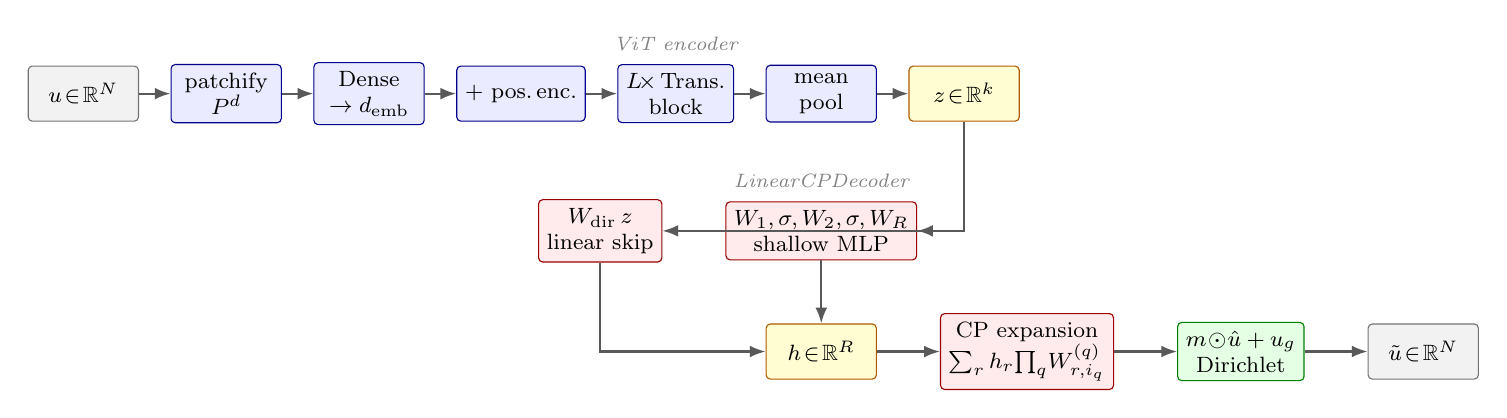
\begin{tikzpicture}[                                                                                   
        font=\footnotesize,                                                                                
        node distance=4mm,                     
        box/.style       ={draw, rounded corners=1.5pt, minimum height=7mm,                                
                           minimum width=14mm, align=center, inner sep=3pt,                                
                           fill=white},        
        enc/.style       ={box, fill=blue!8,  draw=blue!55!black},                                         
        dec/.style       ={box, fill=red!8,   draw=red!60!black},                                          
        io/.style        ={box, fill=gray!10, draw=black!55},                                              
        latent/.style    ={box, fill=yellow!18, draw=orange!70!black},                                     
        mask/.style      ={box, fill=green!10, draw=green!50!black},                                       
        arr/.style       ={-{Latex[length=2mm]}, thick, draw=black!65},                                    
        lbl/.style       ={font=\scriptsize\itshape, gray}                                                 
    ]                                                                                                      
      % ===== ENCODER ROW =====                                                                            
      \node[io]                            (u)     {$u\!\in\!\mathbb{R}^N$};                               
      \node[enc, right=of u]               (patch) {patchify\\$P^d$};                                      
      \node[enc, right=of patch]           (embed) {Dense\\$\to d_\mathrm{emb}$};                          
      \node[enc, right=of embed]           (pos)   {$+$ pos.\,enc.};                                       
      \node[enc, right=of pos]             (vit)   {$L\!\times$\,Trans.\\block};                           
      \node[enc, right=of vit]             (pool)  {mean\\pool};                                           
      \node[latent, right=of pool]         (z)     {$z\!\in\!\mathbb{R}^k$};                               
      \draw[arr] (u)     -- (patch);                                                                       
      \draw[arr] (patch) -- (embed);                                                                       
      \draw[arr] (embed) -- (pos);                                                                         
      \draw[arr] (pos)   -- (vit);                                                                         
      \draw[arr] (vit)   -- (pool);                   
      \draw[arr] (pool)  -- (z);                                                                           
      \node[lbl, above=0.5mm of vit.north] {ViT encoder};                                                  
                                                                                                           
      % ===== DECODER ROW =====                                                                            
      \node[dec,  below=10mm of pool]      (mlp)   {$W_1,\sigma,W_2,\sigma,W_R$\\                          
                                                    shallow MLP};                                          
      \node[dec,  left=8mm of mlp]         (skip)  {$W_\mathrm{dir}\,z$\\
                                                    linear skip};                                          
      \node[latent, below=8mm of mlp]      (h)     {$h\!\in\!\mathbb{R}^R$};
      \node[dec,  right=8mm of h]          (cp)    {CP expansion\\                                         
                                                    $\sum_r h_r\!\prod_q\!W^{(q)}_{r,i_q}$};               
      \node[mask, right=8mm of cp]         (mk)    {$m\!\odot\!\hat u + u_g$\\                             
                                                    Dirichlet};                                            
      \node[io,   right=8mm of mk]         (uout)  {$\tilde u\!\in\!\mathbb{R}^N$};                        
                                                                                                           
      % z splits to both branches                                                                          
      \draw[arr] (z.south) |- (skip.east);                                                                 
      \draw[arr] (z.south) |- (mlp.east);                                                                  
      % branches sum into h                           
      \draw[arr] (skip.south) |- (h.west);                                                                 
      \draw[arr] (mlp.south)  -- (h.north);           
      \draw[arr] (h.east)     -- (cp.west);                                                                
      \draw[arr] (cp.east)    -- (mk.west);                                                                
      \draw[arr] (mk.east)    -- (uout.west);  
                                                                                                           
      \node[lbl, above=0.5mm of mlp.north] {LinearCPDecoder};                                              
    \end{tikzpicture}}                                                                                     
    \caption{NM-ROM pipeline. \textbf{Top:} ViT encoder maps the
      discrete state $u$ to a $k$-dim latent $z$. \textbf{Bottom:}                                                  
      LinearCPDecoder reconstructs $\hat u$ as the sum of a linear skip                                    
      $W_\mathrm{dir}\,z$ and a 2-layer swish MLP fed into a rank-$R$                                      
      canonical-polyadic expansion across the $d$ spatial axes; the                                        
      binary mask $m$ and lift $u_g$ enforce Dirichlet BCs exactly. The                                    
      linear skip keeps $J_\mathcal{D}$ well-conditioned at $z=0$,                                         
      enabling cold-start latent Gauss-Newton.}                                                            
    \label{fig:arch}                                                                                       
  \end{figure}                                                                                             
% =====================================================================
\section{Implementation}
\label{sec:impl}

\subsection{Matrix-free Projected Operators via JAX}

To overcome the bottleneck of explicitly forming the Jacobian
$J_\mathcal{D}$, the framework is implemented utilizing
hardware-accelerated automatic differentiation. The projected
Gauss-Newton operators and time-stepping updates are evaluated
matrix-free using Jacobian-Vector Products (JVPs) and Vector-Jacobian
Products (VJPs) \citep{Bradbury2018JAX}, evaluated strictly over the
hyper-reduced empirical quadrature points. Concretely, JAX gives
\[
  J_\mathcal{D} v \;=\; \mathrm{JVP}(\mathcal{D}, z, v),
  \qquad
  J_\mathcal{D}^\top w \;=\; \mathrm{VJP}(\mathcal{D}, z, w),
\]
and composing the two with one sparse $A \in \{K, M\}$ matvec in
between realises the $k \times k$ Hessian-vector product
$v \mapsto \mathrm{VJP}(\mathcal{D}, z,
A \cdot \mathrm{JVP}(\mathcal{D}, z, v))$,
which we feed to a Krylov solver. The entire pipeline runs on a single
GPU accelerator, with the sparse FD matvec evaluated on the
hyper-reduced support $\mathcal{S}^+$.

\subsection{Training Protocol}

The autoencoder is trained end-to-end by minimising the mean squared
reconstruction error on interior nodes only (boundary nodes are zeroed
by the mask and do not contribute to the loss). The optimiser is AdamW
\citep{LoshchilovHutter2019AdamW} on a warmup-cosine schedule
\citep{LoshchilovHutter2017SGDR}. The
encoder is a Vision Transformer with patch size $8^d$, embedding
dimension $64$, $4$ blocks, and $4$ heads, and the decoder is the
LinearCPDecoder of \S\ref{sec:decoder} with hidden width $256$; these
architectural hyperparameters are fixed across every experiment. The
per-cell training schedule (epochs, batch, peak learning rate, weight
decay, two-stage fine-tuning where applicable) varies with PDE and
resolution and is given in full in
Appendix~\ref{app:training-schedule}; per-cell $k$, $R$, and
$N_\mathrm{eq}$ are reported in Table~\ref{tab:best}. All training
runs on a single NVIDIA A100 GPU.

% =====================================================================
\section{Experimental Setup and Benchmark Problems}
\label{sec:setup}

All full-order models (FOM) and latent non-linear projections are
benchmarked on a single NVIDIA A100 GPU to provide a direct
hardware-to-hardware comparison.

\paragraph{Poisson (elliptic).}
We solve $-\Delta u = 10\sin(k_1 \pi x)\sin(k_2 \pi y)\sin(k_3 \pi z)$
on $[0,1]^d$ with homogeneous Dirichlet boundary conditions, where the
forcing parameters $k_1, k_2, k_3 \sim \mathrm{Uniform}[1, 5]$ are
drawn independently for each training sample. The discrete system uses
a standard finite-difference Laplacian on a uniform structured grid.
Ground-truth solutions are obtained by conjugate gradient on the
discrete stiffness matrix (tolerance $10^{-6}$, up to $5{,}000$
iterations). We evaluate at resolutions $N \in \{64, 128, 256\}$ in
2D and $N \in \{32, 64, 128, 256\}$ in 3D, with $500$ training and
$100$ validation samples. At test time the NM-ROM latent Gauss-Newton
solver starts from $z = 0$ (cold start) with up to $8$ outer iterations
(GN tolerance $10^{-6}$) and a CG inner solver (tolerance $10^{-3}$).

\paragraph{Heat (transient parabolic).}
We solve $\partial_t u - \kappa \Delta u = 0$ on $[0,1]^d$ with
homogeneous Dirichlet boundary conditions, integrating from $t = 0$
to $T = 0.25$ with backward Euler at step size $\Delta t = 0.005$
($50$ steps). The diffusivity $\kappa$ is drawn log-uniformly from
$[0.01, 0.5]$. Initial conditions are superpositions of one to three
Gaussian bumps with centres in $[0.15, 0.85]^d$, amplitudes in
$[1, 10]$, and widths in $[0.05, 0.20]$. We use $500$ training and
$50$ validation trajectories at $N = 64$ ($100$ training, $10$
validation at $N = 128$ due to memory). The NM-ROM uses the same
backward-Euler scheme in the latent space: each step is a
$k \times k$ linear solve with CG (tolerance $10^{-6}$, up to $1{,}000$
iterations), warm-started from the previous latent state.

\paragraph{Metrics.}
We report the relative $L^2$ error
$\|\hat u - u_\mathrm{FOM}\|_2 / \|u_\mathrm{FOM}\|_2$ averaged over
test cases, and the wall-clock speedup
$t_\mathrm{FOM} / t_\mathrm{ROM}$ measured on the same A100 GPU.
For Poisson the FOM time is one CG solve; for Heat it is the full
$50$-step trajectory. The linear POD baseline projects the same
discrete snapshots onto the leading $k$ modes and solves the projected system
exactly (no EQ needed for a linear PDE).

\paragraph{Baselines.}
FNO and DeepONet are re-implemented in JAX/Flax following
\citet{Li2020FNO} and \citet{Lu2021DeepONet} so all baselines run in
the same compute environment as our NM-ROM. We use canonical
configurations from the original works rather than running
independent hyperparameter sweeps per cell --- FNO with width $32$
and $12$ Fourier modes per axis in 2D, width $16$ and $8$ modes in
3D; DeepONet with $500$ uniformly-sampled sensors and a $128$-dim
trunk MLP --- and we acknowledge this in the limitations
(\S\ref{sec:limitations}). SMA-NM-ROM follows the
recipe of \citet{KimChoi2022NMROM} (encoder
$\mathrm{Linear}(m,2m){\to}\mathrm{SiLU}{\to}\mathrm{Linear}(2m,k)$,
mirrored decoder with stencil mask, Adam at $\mathrm{lr}=10^{-3}$,
batch $240$); we report it in \emph{warm-start} mode
($z_0=\mathcal{E}(u_\mathrm{FOM})$, an oracle that already uses the
FOM solution we are trying to predict), because cold-start GN
($z_0=0$, the protocol our NM-ROM uses) diverges to rel-$L^2 \in
[1.4,1.7]$ on every Poisson-2D cell despite the autoencoder
reconstructing validation snapshots at $1.4\%$ — the empirical anchor
for the linear-skip design in \S\ref{sec:decoder}. The SMA-NM-ROM
$m{\times}M_1$ encoder kernel exceeds 40\,GB on a single A100 at
Heat-3D $N{\geq}64$, and on the cells where it does fit the
published backward-Euler latent rollout either explodes (Heat-3D
$N{=}32$: rel-$L^2 \approx 2.6\times 10^{2}$) or runs at
$\leq 0.01\times$ FOM speed (Heat-2D $N{=}64$); the DeepONet
autoregressive rollout overflows to non-finite values on every Heat
cell at $N{\leq}64$ and explodes to rel-$L^2{=}1.25\times 10^{9}$ at
Heat-3D $N{=}128$. These failures are reported as ``---'' in
Table~\ref{tab:operators}.

% =====================================================================


  \section{Numerical Experiments and Results}
  \label{sec:results}                                                                                      
  
  We evaluate NM-ROM against Fourier Neural Operators \citep{Li2020FNO}
  and DeepONets \citep{Lu2021DeepONet}, plus the SMA-NM-ROM baseline
  of \citet{KimChoi2022NMROM}, on the elliptic Poisson and parabolic
  heat equations in 2D and 3D, across eleven (PDE, resolution) cells.
  The framework is implemented in
  JAX \citep{Bradbury2018JAX} for matrix-free automatic differentiation,
  and all full-order baselines and NM-ROM evaluations run on a single
  NVIDIA A100 GPU. Table~\ref{tab:operators} reports the headline
  comparison; the subsections that follow analyse the result along
  three axes (Pareto dominance, per-cell best configurations, and
  which knob to turn).

  \begin{table}[!htbp]
  \centering
  \caption{Best NM-ROM vs.\ FNO, DeepONet, and SMA-NM-ROM
  \citep{KimChoi2022NMROM} at every measured (PDE, $N$) cell. NM-ROM
  \emph{best-acc} (lowest rel-$L^2$) and \emph{best-speed} (highest
  speedup) are deployable from the same trained decoder. Bold marks
  Pareto-dominance over every baseline at the cell. DeepONet rel-$L^2$
  values $\geq 1$ on Poisson indicate the inference output diverging
  from the FOM solution. ``---'' marks cells where the baseline either
  did not run (FNO/DeepONet on Heat-2D $N{=}256$ omitted), the
  autoregressive rollout overflowed to non-finite values
  (DeepONet on every Heat cell), the kernel exceeded 40\,GB on a
  single A100 (SMA-NM-ROM on Heat-3D $N{\geq}64$), or the latent
  rollout exploded above the FOM scale (SMA-NM-ROM on Heat-3D $N{=}32$).
  $^{\dagger}$Poisson-3D rel-$L^2$ are 10-case medians over
  $(k_1,k_2,k_3)\sim\mathcal{U}[1,3]^3$ (LHS, seed=9999). Baseline
  protocols and SMA-NM-ROM warm-start details are in \S\ref{sec:setup}.}
  \label{tab:operators}
  \setlength{\tabcolsep}{3pt}
  \renewcommand{\arraystretch}{1.1}
  \scriptsize
  \begin{tabular}{llcccccccccc}
  \toprule
  & & \multicolumn{2}{c}{NM-ROM best-acc} &
      \multicolumn{2}{c}{NM-ROM best-speed} &
      \multicolumn{2}{c}{FNO} &
      \multicolumn{2}{c}{DeepONet} &
      \multicolumn{2}{c}{SMA-NM-ROM\textsuperscript{$\ddagger$}} \\
  \cmidrule(lr){3-4} \cmidrule(lr){5-6} \cmidrule(lr){7-8}
  \cmidrule(lr){9-10} \cmidrule(lr){11-12}
  PDE & $N$ & rel-$L^2$ & speedup & rel-$L^2$ & speedup
                    & rel-$L^2$ & speedup & rel-$L^2$ & speedup
                    & rel-$L^2$ & speedup \\
  \midrule
  \multirow{3}{*}{Poisson-2D}
    &  64 & 4.84e-3          & \textbf{180}$\times$ & 2.00e-2 & \textbf{324}$\times$ & 4.62e-3 &
  14.5$\times$ & 4.76e-1 & 28.9$\times$ & 1.77e-2 & 15.7$\times$ \\
    & 128 & \textbf{3.23e-3} & \textbf{183}$\times$ & 2.74e-2 & \textbf{321}$\times$ & 7.32e-3 &
  28.5$\times$ & 4.84e-1 & 46.2$\times$ & 1.26e-1 & 11.3$\times$ \\
    & 256 & \textbf{1.35e-3} & \textbf{149}$\times$ & 2.28e-1 & \textbf{295}$\times$ & 7.94e-3 &
  34.3$\times$ & 5.07e-1 & 44.2$\times$ & 3.39e-1 & 8.11$\times$ \\
  \midrule
  \multirow{3}{*}{Poisson-3D$^{\dagger}$}
    &  32 & \textbf{6.94e-3} & \textbf{36.4}$\times$ & 3.21e-1 & \textbf{131}$\times$ & 1.91e-2 &
  5.18$\times$ & 1.60        & 7.67$\times$ & 8.98e-2 & 10.2$\times$ \\
    &  64 & \textbf{6.40e-3} & \textbf{109}$\times$  & 5.88e-2 & \textbf{130}$\times$ & 1.65e-2 &
  4.93$\times$ & 1.22        & 4.64$\times$ & 1.41e-1 & 3.07$\times$ \\
    & 128 & \textbf{1.93e-3} & \textbf{121}$\times$  & 1.39e-2 & \textbf{126}$\times$ & 1.61e-2 &
  3.66$\times$ & 1.19        & 3.06$\times$ & 8.76e-1 & \emph{0.57}$\times$ \\
  \midrule
  \multirow{2}{*}{Heat-2D}
    &  64 & \textbf{5.21e-3} & \textbf{39.6}$\times$  & 1.08e-2 & \textbf{68.0}$\times$  & 1.37e-2     &
  1.60$\times$        & ---        & 7.23$\times$ & 3.09e-1 & \emph{0.01}$\times$ \\
    & 128 & \textbf{3.75e-3} & \textbf{37.8}$\times$  & 1.35e-2 & \textbf{64.2}$\times$  & 5.42e-2     &
  3.38$\times$        & ---        & 23.7$\times$ & ---     & --- \\
  \midrule
  \multirow{3}{*}{Heat-3D}
    &  32 & \textbf{9.30e-2} & \textbf{176}$\times$   & 9.30e-2 & \textbf{176}$\times$   & \textbf{8.17e-2} &
  \emph{0.98}$\times$ & ---         & 9.17$\times$ & ---         & ---                 \\
    &  64 & \textbf{7.49e-2} & \textbf{197}$\times$   & 7.85e-2 & \textbf{269}$\times$   & 2.55e-1     &
  \emph{0.56}$\times$ & ---         & \emph{0.45}$\times$ & ---     & ---                 \\
    & 128 & \textbf{1.82e-1} & \textbf{126}$\times$   & 1.90e-1 & \textbf{191}$\times$   & 2.95e-1     &
  \emph{0.76}$\times$ & ---         & \emph{0.59}$\times$ & ---     & ---                 \\
  \bottomrule
  \end{tabular}
  \\[2pt]
  {\scriptsize \textsuperscript{$\ddagger$}SMA-NM-ROM \citep{KimChoi2022NMROM}
  is reported in \emph{warm-start} mode ($z_0=\mathcal{E}(u_\mathrm{FOM})$,
  an oracle that already uses the FOM solution we are trying to predict);
  cold-start GN ($z_0=0$, the protocol our NM-ROM uses) diverges to
  rel-$L^2 \in [1.4,1.7]$ on every Poisson-2D cell.}
  \end{table}

\subsection{Pareto Dominance over Neural Operators}\label{sec:results:operators}

  For every (PDE, resolution) cell we train one FNO and one DeepONet at
  competitive hyperparameters --- FNO with width $32$ and $12$ Fourier
  modes per axis in 2D, width $16$ and $8$ modes per axis in 3D
  (the canonical configuration of \citet{Li2020FNO}, run on a
  single $80$\,GB A100 to fit the spectral weight tensor at
  $N{=}128^3$), DeepONet with $500$ uniformly-sampled sensors and a
  $128$-dim trunk MLP, both trained until validation rel-$L^2$
  plateaus. Because the headline contribution of NM-ROM is a
  deployment-time accuracy/speed Pareto curve traced by a single
  trained model, the comparison against fixed-point baselines is
  presented as two extremes of that curve rather than a single number:
  three deployment-time knobs (GN iteration cap, GN early-exit
  tolerance, EQ sample count) move continuously between
  \emph{best-accuracy} (lowest rel-$L^2$) and \emph{best-speedup}
  (highest wall-clock ratio over full-order CG), both evaluated from
  the same trained decoder.
                                                                                                           
  \paragraph{NM-ROM Pareto-dominates both baselines on 10 of 11 cells.}
  At every measured (PDE, resolution) cell except Poisson-2D
  $N{=}64$, at least one NM-ROM point has lower rel-$L^2$
  \emph{and} higher speedup than every baseline
  (Table~\ref{tab:operators}, bold); on the one exception NM-ROM is
  marginally less accurate than FNO ($4.84{\rm e}{-3}$ vs.\
  $4.62{\rm e}{-3}$) but $12\times$ faster, and runs $22\times$
  faster still at its best-speed point. The gap is largest where the
  solution manifold is most non-linear (Poisson-3D) and at the
  highest resolutions, where the asymptotic FOM cost grows faster
  than the EQ-bounded ROM. The most extreme cell is Heat-3D
  $N{=}128$: NM-ROM reaches rel-$L^2 = 1.82\times 10^{-1}$ at
  $191\times$ speedup, while FNO is slower than FOM
  ($0.76\times$) at $2.95\times 10^{-1}$ and DeepONet's
  autoregressive rollout explodes (rel-$L^2 = 1.25\times 10^{9}$).
  Per cell, NM-ROM exposes between $13$ and $39$ trained-once,
  deployment-tunable Pareto points; FNO and DeepONet expose one
  fixed point each.

  \subsection{Best Configurations per Problem and Resolution}
  \label{sec:results:best}
                                                                                                           
  Table~\ref{tab:best} reports the trained-once best-accuracy and                                          
  best-speed NM-ROM configurations at each (problem, resolution) pair.                                     
  Latent dimension $k$, CP rank $R$, and EQ sample count $N_\mathrm{eq}$                                   
  are problem-dependent; all other architectural hyperparameters
  (\S\ref{sec:decoder}, \S\ref{sec:impl}) are fixed across every
  cell.                                                                                                    
                                                                                                           
  \begin{table}[!htbp]
  \centering
  \caption{Trained-once NM-ROM configurations. Each row gives the
  \emph{best-accuracy / best-speed} values from the same trained
  decoder. $k$: latent dim; $R$: CP rank; $N_\mathrm{eq}$: EQ-selected
  nodes (``---'': full residual). Pairs collapse to a single value
  when best-acc and best-speed coincide.}
  \label{tab:best}
  \setlength{\tabcolsep}{5pt}
  \small
  \begin{tabular}{lcccll}
  \toprule
  Cell & $k$ & $R$ & $N_\mathrm{eq}$ & rel-$L^2$ (acc / speed) & Speedup (acc / speed) \\
  \midrule
  Poisson-2D, $N{=}64$  & 8  & 128 & 640  & 4.84e-3 / 2.00e-2 & 180$\times$\,/\,324$\times$ \\
  Poisson-2D, $N{=}128$ & 12 & 768/512 & 960  & 3.23e-3 / 2.74e-2 & 183$\times$\,/\,321$\times$ \\
  Poisson-2D, $N{=}256$ & 16 & 768/512 & 1280 & 1.35e-3 / 2.28e-1 & 149$\times$\,/\,295$\times$ \\
  Poisson-3D, $N{=}32$  & 24/8 & 512/128 & --- & 6.94e-3 / 3.21e-1 & 36.4$\times$\,/\,131$\times$ \\
  Poisson-3D, $N{=}64$  & 16 & 512 & 600  & 6.40e-3 / 7.69e-3 & 109$\times$\,/\,130$\times$ \\
  Poisson-3D, $N{=}128$ & 16 & 768/512 & 2000/1000 & 1.93e-3 / 1.39e-2 & 121$\times$\,/\,126$\times$ \\
  Heat-2D, $N{=}64$     & 64 & 256 & --- & 5.21e-3 / 1.08e-2 & 39.6$\times$\,/\,68.0$\times$ \\
  Heat-2D, $N{=}128$    & 64 & 256 & --- & 3.75e-3 / 1.35e-2 & 37.8$\times$\,/\,64.2$\times$ \\
  Heat-3D, $N{=}32$     & 32 & 512 & 512 & 9.30e-2           & 176$\times$ \\
  Heat-3D, $N{=}64$     & 40 & 512 & 2560 & 7.49e-2 / 7.85e-2 & 197$\times$\,/\,269$\times$ \\
  Heat-3D, $N{=}128$    & 40 & 512 & 1280 & 1.82e-1 / 1.90e-1 & 126$\times$\,/\,191$\times$ \\
  \bottomrule
  \end{tabular}
  \end{table}                                                                                              
                                                      
  The same trained decoder serves both axes. Going from best-accuracy to                                   
  best-speed within a cell never requires retraining --- only the GN
  iteration cap, GN tolerance, and EQ sample count change. This is what                                    
  we mean by deployment-time tunability: a single training run produces                                    
  a continuous Pareto frontier, of which best-acc and best-speed are                                       
  the two extremes.                                                                                        
                                                                                                           
  \subsection{Pareto Navigation: Which Knob to Turn}                                                       
  \label{sec:results:tunability}                      
                                                                                                           
  We classify each tunable knob in our framework into three groups: (i)                                    
  \emph{deployment-time} knobs that walk the Pareto without retraining,
  (ii) \emph{training-time accuracy} knobs that push the achievable                                        
  frontier downward, and (iii) \emph{engineering} knobs (binary on/off,                                    
  no accuracy effect, large speedup contribution). Tables~\ref{tab:t2a}                                    
  and \ref{tab:t2b} list the directional findings, mined from per-run                                      
  notes across our autoresearch logs. Knobs without a consistent                                           
  direction on a given axis are excluded from that table.                                                  
                                                                                                           
  \begin{table}[!htbp]                                                                                         
  \centering                                                                                               
  \caption{Knobs that push \emph{accuracy}. Direction is the way to
  turn the knob to lower rel-$L^2$. Evidence column cites the                                              
  autoresearch run that established the direction.}                                                        
  \label{tab:t2a}                                                                                          
  \small                                                                                                   
  \setlength{\tabcolsep}{4pt}                         
  \begin{tabular}{p{3.0cm}p{2.4cm}p{1.4cm}p{5.5cm}}                                                        
  \toprule                                                                                                 
  Knob & Range & Direction & Evidence \\       
  \midrule                                                                                                 
  Latent dim $k$         & $\{4..64\}$        & $\uparrow$ to PDE-specific sweet spot
    & P3D N=64: $k{=}20$ GN diverges; H2D N=128: $k{=}64$ best. \\                                         
  GN max iters           & $\{3..50\}$        & $\uparrow$                                                 
    & H2D N=128: max\_iters$=8 \to 15$ takes rel-$L^2$ $2.3{\rm e}{-2} \to 1.3{\rm e}{-2}$. \\             
  GN tolerance           & $\{10^{-2}..10^{-1}\}$ & $\downarrow$                                           
    & P3D N=128 Run3: tol $5{\rm e}{-2} \to 1{\rm e}{-4}$ improves accuracy at the cost of iters. \\       
  EQ samples $n_\mathrm{eq}$ & $\{4..64\}$    & $\uparrow$                                                 
    & H3D N=64: $n_\mathrm{eq}=32 \to 64$ doubles coverage at no accuracy cost. \\                         
  \bottomrule                                                                                              
  \end{tabular}                                                                                            
  \end{table}                                                                                              
                                                                                                           
  \begin{table}[!htbp]                             
  \centering                                                                                               
  \caption{Knobs that push \emph{speedup}. Direction is the way to turn
  the knob to increase wall-clock speedup. The first three rows are
  deployment-time knobs (no retraining); the last three are engineering                                    
  optimizations.}
  \label{tab:t2b}                                                                                          
  \small                                              
  \setlength{\tabcolsep}{4pt}                                                                              
  \begin{tabular}{p{3.0cm}p{2.4cm}p{1.4cm}p{5.5cm}}
  \toprule                                                                                                 
  Knob & Range & Direction & Evidence \\                                                                   
  \midrule                                     
  \multicolumn{4}{l}{\emph{Deployment-time (no retraining):}} \\                                           
  GN max iters           & $\{3..50\}$        & $\downarrow$                                               
    & P3D N=64: max\_iters $20 \to 11$ takes speedup $51 \to 96\times$ at same accuracy. \\                
  GN tolerance           & $\{10^{-2}..10^{-1}\}$ & $\uparrow$ (looser)                                    
    & P3D N=128 Run3: tol $1{\rm e}{-4} \to 5{\rm e}{-2}$ takes speedup $57 \to 109\times$. \\             
  EQ samples $n_\mathrm{eq}$ & $\{4..64\}$    & $\downarrow$                                               
    & H3D N=32 Run12: $n_\mathrm{eq}=4$ extends speedup frontier. \\                                       
  \bottomrule                                                                                              
  \end{tabular}                                                                                            
  \end{table}                                                                                              
                                                                                                           
  The deployment-time row of Table~\ref{tab:t2b} is what makes NM-ROM                                      
  \emph{tunable} in a way neural operators are not: the same trained                                       
  decoder is reused, only solver-side knobs change. The training-time                                      
  knobs in Table~\ref{tab:t2a} push the achievable frontier downward                                       
  but require a fresh training run per setting. The engineering row of                                     
  Table~\ref{tab:t2b} contributes the bulk of our best-speedup numbers                                     
  on Heat-3D --- in particular, the $\kappa$-as-runtime-arg JAX-tracing                                    
  fix on its own takes the trained Heat-3D $N=128$ model from $14.7\times$                                 
  to $191\times$ wall-clock, with bit-identical accuracy.                                                  
                                                                                                           
\FloatBarrier
% =====================================================================
\paragraph{Limitations.}
\label{sec:limitations}
(i) All cells are evaluated at a single random seed; we do not
report variance across runs. (ii) Discretisations are
finite-difference on uniform Cartesian grids; transfer to unstructured
FEM meshes and curved geometries is untested and we expect the CP
spatial head to require modification. (iii) Benchmarks are restricted
to the elliptic Poisson and parabolic heat equations; advection-dominated
problems (Burgers, shallow water, wave) are not evaluated and would
exercise solver-side machinery our framework does not currently
include. (iv) Baseline hyperparameters are taken from canonical
configurations rather than independently re-swept per cell.
(v) Heat rollouts are 50 steps; long-horizon stability beyond this
window is not assessed. (vi) Training cost ranges from $\sim$10
minutes (Poisson-3D $N{=}64$) to $\sim$8 hours (Heat-2D $N{=}128$,
$300{,}000$ epochs) on a single A100; the amortisation argument is
implicit in many-query deployment.

% =====================================================================
\section{Conclusion and Future Work}
\label{sec:conclusion}

We built an NM-ROM for elliptic and parabolic PDEs whose distinguishing
property is a deployment-time accuracy/speed Pareto curve traced by a
single trained model: at inference, three solver-side knobs --- the
Gauss-Newton iteration cap, the Gauss-Newton early-exit tolerance, and
the Empirical Quadrature sample count --- continuously trade accuracy
for speedup. This is the lever neural operators do not expose: each
trained FNO or DeepONet delivers one fixed operating point. The
framework is faster than full-order conjugate gradient and beats both
neural-operator baselines on accuracy and speed at every measured cell
except one. Mechanically, the decoder is a learned non-linear manifold
that lifts the Kolmogorov $n$-width barrier of linear POD; the PDE
itself is enforced by Galerkin projection of the discrete residual onto
that manifold; Dirichlet boundary conditions are enforced exactly by a
binary mask in the decoder; Empirical Quadrature decouples residual
cost from mesh size; and the whole pipeline is matrix-free in JAX.

Three pieces had to come together to make this work. First, an
architectural choice --- the LinearCPDecoder (linear skip + shallow MLP
+ rank-$R$ canonical-polyadic head) feeding from a ViT encoder --- that
simultaneously satisfies the cold-start Gauss-Newton convergence,
EQ-compatibility, and sub-cubic parameter-scaling constraints that
prior NM-ROM decoders could not satisfy together at 3D resolution.
Second, exact Dirichlet enforcement by decoder masking, which lets the
Galerkin projection annihilate boundary equations as in classical
projection methods rather than via soft penalties. Third, a JAX
implementation that evaluates every projected operator matrix-free
through forward- and reverse-mode automatic differentiation, removing
the dense-Jacobian bottleneck that historically pinned NM-ROMs to
small problems.

Across the elliptic Poisson and parabolic heat equations in 2D and 3D
the framework delivers wall-clock speedups over full-order conjugate
gradient from $36\times$ to $324\times$ at engineering-grade accuracy.
A natural next step is to evaluate the same framework on
advection-dominated benchmarks --- 1D and 2D Burgers, shallow water
--- where the $n$-width gap between linear and non-linear manifolds is
largest, and where existing neural operators also tend to be
unreliable. Extending the spatial head beyond Cartesian tensor
products to support unstructured meshes is a second open direction.

% =====================================================================
\bibliographystyle{plainnat}
\begin{thebibliography}{99}

\bibitem[Barnett and Farhat(2022)]{BarnettFarhat2022}
J.~Barnett and C.~Farhat.
\newblock Quadratic approximation manifold for mitigating the
Kolmogorov barrier in nonlinear projection-based model order reduction.
\newblock \emph{Journal of Computational Physics}, 464:111348, 2022.
\bibitem[Benner et~al.(2015)]{BennerGugercinWillcox2015}
P.~Benner, S.~Gugercin, and K.~Willcox.
\newblock A survey of projection-based model reduction methods for
parametric dynamical systems.
\newblock \emph{SIAM Review}, 57(4):483--531, 2015.

\bibitem[Berkooz et~al.(1993)]{Berkooz1993}
G.~Berkooz, P.~Holmes, and J.~L. Lumley.
\newblock The proper orthogonal decomposition in the analysis of
turbulent flows.
\newblock \emph{Annual Review of Fluid Mechanics}, 25(1):539--575, 1993.

\bibitem[Berrone et~al.(2022)]{BerroneBC2022}
S.~Berrone, C.~Canuto, M.~Pintore, and N.~Sukumar.
\newblock Enforcing Dirichlet boundary conditions in physics-informed
neural networks and variational physics-informed neural networks.
\newblock \emph{arXiv preprint arXiv:2210.14795}, 2022.

\bibitem[Boull\'e and Townsend(2024)]{BoulleTownsend2024}
N.~Boull\'e and A.~Townsend.
\newblock A mathematical guide to operator learning.
\newblock In \emph{Handbook of Numerical Analysis}, volume~25, pages
83--125. Elsevier, 2024.

\bibitem[Bradbury et~al.(2018)]{Bradbury2018JAX}
J.~Bradbury, R.~Frostig, P.~Hawkins, M.~J. Johnson, C.~Leary,
D.~Maclaurin, G.~Necula, A.~Paszke, J.~VanderPlas, S.~Wanderman-Milne,
and Q.~Zhang.
\newblock JAX: composable transformations of Python+NumPy programs, 2018.

\bibitem[Brecht et~al.(2023)]{BrechtHardConstraints2023}
R.~Brecht, R.~O. Popovych, A.~Bihlo, and Y.~Popovych.
\newblock Improving physics-informed DeepONets with hard constraints.
\newblock \emph{arXiv preprint arXiv:2309.07899}, 2023.

\bibitem[Cai et~al.(2020)]{Cai2020OnceForAll}
H.~Cai, C.~Gan, T.~Wang, Z.~Zhang, and S.~Han.
\newblock Once-for-All: Train one network and specialize it for
efficient deployment.
\newblock In \emph{International Conference on Learning Representations},
2020.

\bibitem[Cao(2021)]{Cao2021GalerkinTransformer}
S.~Cao.
\newblock Choose a Transformer: Fourier or Galerkin.
\newblock In \emph{Advances in Neural Information Processing Systems},
2021.

\bibitem[Carlberg et~al.(2011)]{Carlberg2011LSPG}
K.~Carlberg, C.~Bou-Mosleh, and C.~Farhat.
\newblock Efficient non-linear model reduction via a least-squares
Petrov--Galerkin projection and compressive tensor approximations.
\newblock \emph{International Journal for Numerical Methods in
Engineering}, 86(2):155--181, 2011.

\bibitem[Chaturantabut and Sorensen(2010)]{ChaturantabutSorensen2010}
S.~Chaturantabut and D.~C. Sorensen.
\newblock Nonlinear model reduction via discrete empirical
interpolation.
\newblock \emph{SIAM Journal on Scientific Computing}, 32(5):2737--2764,
2010.

\bibitem[Chen et~al.(2024)]{Chen2024UnsupervisedNO}
W.~Chen, J.~Song, P.~Ren, S.~Subramanian, D.~Morozov, and M.~W.
Mahoney.
\newblock Data-efficient operator learning via unsupervised pretraining
and in-context learning.
\newblock In \emph{Advances in Neural Information Processing Systems},
2024.

\bibitem[Cohen and DeVore(2015)]{CohenDeVore2015}
A.~Cohen and R.~DeVore.
\newblock Approximation of high-dimensional parametric PDEs.
\newblock \emph{Acta Numerica}, 24:1--159, 2015.

\bibitem[Diaz et~al.(2024)]{Diaz2024DomainDecompNMROM}
A.~N. Diaz, Y.~Choi, and M.~Heinkenschloss.
\newblock A fast and accurate domain-decomposition nonlinear manifold
reduced order model.
\newblock \emph{Computer Methods in Applied Mechanics and Engineering},
425:116943, 2024.

\bibitem[Dosovitskiy et~al.(2021)]{Dosovitskiy2021ViT}
A.~Dosovitskiy, L.~Beyer, A.~Kolesnikov, D.~Weissenborn, X.~Zhai,
T.~Unterthiner, M.~Dehghani, M.~Minderer, G.~Heigold, S.~Gelly,
J.~Uszkoreit, and N.~Houlsby.
\newblock An image is worth 16x16 words: Transformers for image
recognition at scale.
\newblock In \emph{International Conference on Learning Representations},
2021.

\bibitem[Eshaghi et~al.(2025)]{EshaghiNOWS2025}
M.~S. Eshaghi, C.~Anitescu, N.~Valizadeh, Y.~Wang, X.~Zhuang, and
T.~Rabczuk.
\newblock NOWS: Neural operator warm starts for accelerating iterative
solvers.
\newblock \emph{arXiv preprint arXiv:2511.02481}, 2025.

\bibitem[Farhat et~al.(2014)]{FarhatECSW2014}
C.~Farhat, P.~Avery, T.~Chapman, and J.~Cortial.
\newblock Dimensional reduction of nonlinear finite element dynamic
models with finite rotations and energy-based mesh sampling and
weighting for computational efficiency.
\newblock \emph{International Journal for Numerical Methods in
Engineering}, 98(9):625--662, 2014.

\bibitem[Fresca and Manzoni(2022)]{FrescaManzoni2022PODDLROM}
S.~Fresca and A.~Manzoni.
\newblock POD-DL-ROM: Enhancing deep learning-based reduced order
models for nonlinear parametrized PDEs by proper orthogonal decomposition.
\newblock \emph{Computer Methods in Applied Mechanics and Engineering},
388:114181, 2022.

\bibitem[Geelen et~al.(2022)]{GeelenWrightWillcox2022}
R.~Geelen, S.~Wright, and K.~Willcox.
\newblock Operator inference for non-intrusive model reduction with
quadratic manifolds.
\newblock \emph{Computer Methods in Applied Mechanics and Engineering},
403:115717, 2022.

\bibitem[Greif and Urban(2019)]{GreifUrban2019}
C.~Greif and K.~Urban.
\newblock Decay of the Kolmogorov $N$-width for wave problems.
\newblock \emph{Applied Mathematics Letters}, 96:216--222, 2019.

\bibitem[Griewank and Walther(2008)]{GriewankWalther2008}
A.~Griewank and A.~Walther.
\newblock \emph{Evaluating Derivatives: Principles and Techniques of
Algorithmic Differentiation}.
\newblock SIAM, Philadelphia, 2nd edition, 2008.

\bibitem[Hao et~al.(2023)]{HaoGNOT2023}
Z.~Hao, Z.~Wang, H.~Su, C.~Ying, Y.~Dong, S.~Liu, Z.~Cheng, J.~Song,
and J.~Zhu.
\newblock GNOT: A general neural operator transformer for operator
learning.
\newblock In \emph{International Conference on Machine Learning}, 2023.

\bibitem[Hao et~al.(2024)]{HaoDPOT2024}
Z.~Hao, C.~Su, S.~Liu, J.~Berner, C.~Ying, H.~Su, A.~Anandkumar,
J.~Song, and J.~Zhu.
\newblock DPOT: Auto-regressive denoising operator transformer for
large-scale PDE pre-training.
\newblock In \emph{International Conference on Machine Learning}, 2024.

\bibitem[Herde et~al.(2024)]{HerdePoseidon2024}
M.~Herde, B.~Raonic, T.~Rohner, R.~K\"appeli, R.~Molinaro,
E.~de~Bezenac, and S.~Mishra.
\newblock Poseidon: Efficient foundation models for PDEs.
\newblock In \emph{Advances in Neural Information Processing Systems},
2024.

\bibitem[Hern\'andez et~al.(2017)]{Hernandez2017EQ}
J.~A. Hern\'andez, M.~A. Caicedo, and A.~Ferrer.
\newblock Dimensional hyper-reduction of nonlinear finite element
models via empirical cubature.
\newblock \emph{Computer Methods in Applied Mechanics and Engineering},
313:687--722, 2017.

\bibitem[Hestenes and Stiefel(1952)]{HestenesStiefel1952CG}
M.~R. Hestenes and E.~Stiefel.
\newblock Methods of conjugate gradients for solving linear systems.
\newblock \emph{Journal of Research of the National Bureau of Standards},
49(6):409--436, 1952.

\bibitem[Hesthaven et~al.(2016)]{HesthavenRozzaStamm2016}
J.~S. Hesthaven, G.~Rozza, and B.~Stamm.
\newblock \emph{Certified Reduced Basis Methods for Parametrized
Partial Differential Equations}.
\newblock SpringerBriefs in Mathematics. Springer, 2016.

\bibitem[Hirsch et~al.(2024)]{HirschPichiHesthavenNEIM2024}
M.~Hirsch, F.~Pichi, and J.~S. Hesthaven.
\newblock Neural empirical interpolation method for nonlinear model
reduction.
\newblock \emph{arXiv preprint arXiv:2406.03562}, 2024.

\bibitem[Holzschuh et~al.(2025)]{HolzschuhPDETransformer2025}
B.~Holzschuh, Q.~Liu, G.~Kohl, and N.~Thuerey.
\newblock PDE-Transformer: Efficient and versatile transformers for
physics simulations.
\newblock In \emph{International Conference on Machine Learning}, 2025.

\bibitem[Hu et~al.(2025)]{HuLinearNO2025}
W.~Hu, S.~Liu, P.~Qiao, Z.~Sun, and Y.~Dou.
\newblock Transolver is a linear transformer: Revisiting
physics-attention through the lens of linear attention.
\newblock \emph{arXiv preprint arXiv:2511.06294}, 2025.

\bibitem[Hughes(2000)]{Hughes2000FEM}
T.~J.~R. Hughes.
\newblock \emph{The Finite Element Method: Linear Static and Dynamic
Finite Element Analysis}.
\newblock Dover Publications, 2000.

\bibitem[Karniadakis et~al.(2021)]{Karniadakis2021PIML}
G.~E. Karniadakis, I.~G. Kevrekidis, L.~Lu, P.~Perdikaris, S.~Wang, and
L.~Yang.
\newblock Physics-informed machine learning.
\newblock \emph{Nature Reviews Physics}, 3:422--440, 2021.

\bibitem[Kim et~al.(2022)]{KimChoi2022NMROM}
Y.~Kim, Y.~Choi, D.~Widemann, and T.~Zohdi.
\newblock A fast and accurate physics-informed neural network reduced
order model with shallow masked autoencoder.
\newblock \emph{Journal of Computational Physics}, 451:110841, 2022.

\bibitem[Kim et~al.(2024)]{KimWenLeeChoiCNFROM2024}
M.~Kim, T.~Wen, K.~Lee, and Y.~Choi.
\newblock Physics-informed reduced order model with conditional neural
fields.
\newblock \emph{arXiv preprint arXiv:2412.05233}, 2024.

\bibitem[Kochkov et~al.(2021)]{Kochkov2021PNAS}
D.~Kochkov, J.~A. Smith, A.~Alieva, Q.~Wang, M.~P. Brenner, and
S.~Hoyer.
\newblock Machine learning--accelerated computational fluid dynamics.
\newblock \emph{Proceedings of the National Academy of Sciences},
118(21):e2101784118, 2021.

\bibitem[Kolda and Bader(2009)]{KoldaBader2009CP}
T.~G. Kolda and B.~W. Bader.
\newblock Tensor decompositions and applications.
\newblock \emph{SIAM Review}, 51(3):455--500, 2009.

\bibitem[Kopani\v{c}\'akov\'a and Karniadakis(2024)]{KopanicakovaKarniadakis2024}
A.~Kopani\v{c}\'akov\'a and G.~E. Karniadakis.
\newblock DeepOnet based preconditioning strategies for solving
parametric linear systems of equations.
\newblock \emph{arXiv preprint arXiv:2401.02016}, 2024.

\bibitem[Kovachki et~al.(2023)]{Kovachki2023NeuralOperator}
N.~Kovachki, Z.~Li, B.~Liu, K.~Azizzadenesheli, K.~Bhattacharya,
A.~Stuart, and A.~Anandkumar.
\newblock Neural operator: learning maps between function spaces.
\newblock \emph{Journal of Machine Learning Research}, 24(89):1--97,
2023.

\bibitem[Lawson and Hanson(1974)]{LawsonHanson1974NNLS}
C.~L. Lawson and R.~J. Hanson.
\newblock \emph{Solving Least Squares Problems}.
\newblock Prentice-Hall, Englewood Cliffs, NJ, 1974.

\bibitem[Lee and Carlberg(2020)]{LeeCarlberg2020}
K.~Lee and K.~T. Carlberg.
\newblock Model reduction of dynamical systems on nonlinear manifolds
using deep convolutional autoencoders.
\newblock \emph{Journal of Computational Physics}, 404:108973, 2020.

\bibitem[Li et~al.(2021)]{Li2020FNO}
Z.~Li, N.~Kovachki, K.~Azizzadenesheli, B.~Liu, K.~Bhattacharya,
A.~Stuart, and A.~Anandkumar.
\newblock Fourier neural operator for parametric partial differential
equations.
\newblock In \emph{International Conference on Learning Representations},
2021.

\bibitem[Li et~al.(2023a)]{LiGeoFNO2023}
Z.~Li, D.~Z. Huang, B.~Liu, and A.~Anandkumar.
\newblock Fourier neural operator with learned deformations for PDEs
on general geometries.
\newblock \emph{Journal of Machine Learning Research}, 24(388):1--26,
2023.

\bibitem[Li et~al.(2023b)]{LiOFormer2023}
Z.~Li, K.~Meidani, and A.~B. Farimani.
\newblock Transformer for partial differential equations' operator
learning.
\newblock \emph{Transactions on Machine Learning Research}, 2023.

\bibitem[Li et~al.(2024)]{Li2024PINO}
Z.~Li, H.~Zheng, N.~Kovachki, D.~Jin, H.~Chen, B.~Liu,
K.~Azizzadenesheli, and A.~Anandkumar.
\newblock Physics-informed neural operator for learning partial
differential equations.
\newblock \emph{ACM/IMS Journal of Data Science}, 1(3):1--27, 2024.

\bibitem[Lippe et~al.(2023)]{LippePDERefiner2023}
P.~Lippe, B.~Veeling, P.~Perdikaris, R.~E. Turner, and J.~Brandstetter.
\newblock PDE-Refiner: Achieving accurate long rollouts with neural
PDE solvers.
\newblock In \emph{Advances in Neural Information Processing Systems},
2023.

\bibitem[Loshchilov and Hutter(2017)]{LoshchilovHutter2017SGDR}
I.~Loshchilov and F.~Hutter.
\newblock SGDR: Stochastic gradient descent with warm restarts.
\newblock In \emph{International Conference on Learning Representations},
2017.

\bibitem[Loshchilov and Hutter(2019)]{LoshchilovHutter2019AdamW}
I.~Loshchilov and F.~Hutter.
\newblock Decoupled weight decay regularization.
\newblock In \emph{International Conference on Learning Representations},
2019.

\bibitem[Luo et~al.(2016)]{Luo2016ERF}
W.~Luo, Y.~Li, R.~Urtasun, and R.~Zemel.
\newblock Understanding the effective receptive field in deep
convolutional neural networks.
\newblock In \emph{Advances in Neural Information Processing Systems},
2016.

\bibitem[Lu et~al.(2021)]{Lu2021DeepONet}
L.~Lu, P.~Jin, G.~Pang, Z.~Zhang, and G.~E. Karniadakis.
\newblock Learning nonlinear operators via DeepONet based on the
universal approximation theorem of operators.
\newblock \emph{Nature Machine Intelligence}, 3(3):218--229, 2021.

\bibitem[McCabe et~al.(2024)]{McCabeMPP2024}
M.~McCabe, B.~R\'egaldo-Saint Blancard, L.~H. Parker, R.~Ohana,
M.~Cranmer, A.~Bietti, M.~Eickenberg, S.~Golkar, G.~Krawezik,
F.~Lanusse, M.~Pettee, T.~Tesileanu, K.~Cho, and S.~Ho.
\newblock Multiple physics pretraining for physical surrogate models.
\newblock In \emph{Advances in Neural Information Processing Systems},
2024.

\bibitem[Mirhoseini and Zahr(2023)]{MirhoseiniZahr2023}
M.~A. Mirhoseini and M.~J. Zahr.
\newblock Accelerated solutions of convection-dominated partial
differential equations using implicit feature tracking and empirical
quadrature.
\newblock \emph{arXiv preprint arXiv:2305.15661}, 2023.

\bibitem[Negri et~al.(2015)]{NegriManzoniAmsallem2015}
F.~Negri, A.~Manzoni, and D.~Amsallem.
\newblock Efficient model reduction of parametrized systems by matrix
discrete empirical interpolation.
\newblock \emph{Journal of Computational Physics}, 303:431--454, 2015.

\bibitem[Nguyen(2024)]{Nguyen2024HighOrderEIM}
N.~C. Nguyen.
\newblock High-order empirical interpolation methods for real time
solution of parametrized nonlinear PDEs.
\newblock \emph{arXiv preprint arXiv:2410.02100}, 2024.

\bibitem[Nocedal and Wright(2006)]{NocedalWright2006}
J.~Nocedal and S.~J. Wright.
\newblock \emph{Numerical Optimization}.
\newblock Springer Series in Operations Research and Financial
Engineering. Springer, New York, 2nd edition, 2006.

\bibitem[Novikov et~al.(2015)]{Novikov2015TT}
A.~Novikov, D.~Podoprikhin, A.~Osokin, and D.~P. Vetrov.
\newblock Tensorizing neural networks.
\newblock In \emph{Advances in Neural Information Processing Systems},
2015.

\bibitem[Ohlberger and Rave(2016)]{OhlbergerRave2016}
M.~Ohlberger and S.~Rave.
\newblock Reduced basis methods: success, limitations and future
challenges.
\newblock In \emph{Proceedings of the ALGORITMY Conference}, 2016.

\bibitem[Quarteroni et~al.(2015)]{QuarteroniManzoniNegri2015}
A.~Quarteroni, A.~Manzoni, and F.~Negri.
\newblock \emph{Reduced Basis Methods for Partial Differential
Equations: An Introduction}.
\newblock UNITEXT, Vol.~92. Springer, 2015.

\bibitem[Raissi et~al.(2019)]{Raissi2019}
M.~Raissi, P.~Perdikaris, and G.~E. Karniadakis.
\newblock Physics-informed neural networks.
\newblock \emph{Journal of Computational Physics}, 378:686--707, 2019.

\bibitem[Romor et~al.(2023)]{RomorStabileRozza2023}
F.~Romor, G.~Stabile, and G.~Rozza.
\newblock Non-linear manifold reduced-order models with convolutional
autoencoders and reduced over-collocation method.
\newblock \emph{Journal of Scientific Computing}, 94:74, 2023.

\bibitem[Saad(2003)]{Saad2003}
Y.~Saad.
\newblock \emph{Iterative Methods for Sparse Linear Systems}.
\newblock SIAM, Philadelphia, 2nd edition, 2003.

\bibitem[Shikhman(2026)]{Shikhman2026BoundaryIndexed}
L.~J. Shikhman.
\newblock One operator to rule them all? On boundary-indexed operator
families in neural PDE solvers.
\newblock \emph{arXiv preprint arXiv:2603.01406}, 2026.

\bibitem[Sirovich(1987)]{Sirovich1987POD}
L.~Sirovich.
\newblock Turbulence and the dynamics of coherent structures, Parts
I--III.
\newblock \emph{Quarterly of Applied Mathematics}, 45(3):561--590, 1987.

\bibitem[Sukumar and Srivastava(2022)]{SukumarSrivastava2022}
N.~Sukumar and A.~Srivastava.
\newblock Exact imposition of boundary conditions with distance
functions in physics-informed deep neural networks.
\newblock \emph{Computer Methods in Applied Mechanics and Engineering},
389:114333, 2022.

\bibitem[Tran et~al.(2023)]{TranFFNO2023}
A.~Tran, A.~Mathews, L.~Xie, and C.~S. Ong.
\newblock Factorized Fourier neural operators.
\newblock In \emph{International Conference on Learning Representations},
2023.

\bibitem[Um et~al.(2020)]{UmSolverInTheLoop2020}
K.~Um, R.~Brand, Y.~Fei, P.~Holl, and N.~Thuerey.
\newblock Solver-in-the-loop: Learning from differentiable physics to
interact with iterative PDE-solvers.
\newblock In \emph{Advances in Neural Information Processing Systems},
2020.

\bibitem[Vaswani et~al.(2017)]{Vaswani2017Attention}
A.~Vaswani, N.~Shazeer, N.~Parmar, J.~Uszkoreit, L.~Jones, A.~N. Gomez,
\L.~Kaiser, and I.~Polosukhin.
\newblock Attention is all you need.
\newblock In \emph{Advances in Neural Information Processing Systems},
2017.

\bibitem[Virtanen et~al.(2020)]{Virtanen2020SciPy}
P.~Virtanen, R.~Gommers, T.~E. Oliphant, M.~Haberland, T.~Reddy,
D.~Cournapeau, E.~Burovski, P.~Peterson, W.~Weckesser, J.~Bright, S.~J.
van~der Walt, M.~Brett, J.~Wilson, K.~J. Millman, N.~Mayorov, A.~R.~J.
Nelson, E.~Jones, R.~Kern, E.~Larson, C.~J. Carey, \.I.~Polat, Y.~Feng,
E.~W. Moore, J.~VanderPlas, D.~Laxalde, J.~Perktold, R.~Cimrman,
I.~Henriksen, E.~A. Quintero, C.~R. Harris, A.~M. Archibald, A.~H.
Ribeiro, F.~Pedregosa, P.~van Mulbregt, and SciPy~1.0 Contributors.
\newblock SciPy 1.0: Fundamental algorithms for scientific computing
in Python.
\newblock \emph{Nature Methods}, 17(3):261--272, 2020.

\bibitem[Wen et~al.(2025)]{WenGAOT2025}
S.~Wen, A.~Kumbhat, L.~Lingsch, S.~Mousavi, Y.~Zhao, P.~Chandrashekar,
and S.~Mishra.
\newblock Geometry aware operator transformer as an efficient and
accurate neural surrogate for PDEs on arbitrary domains.
\newblock In \emph{Advances in Neural Information Processing Systems},
2025.

\bibitem[Wang and Wang(2024)]{WangLNO2024}
T.~Wang and C.~Wang.
\newblock Latent neural operator for solving forward and inverse PDE
problems.
\newblock In \emph{Advances in Neural Information Processing Systems},
2024.

\bibitem[Wang et~al.(2024)]{WangBENO2024}
H.~Wang, J.~Li, A.~Dwivedi, K.~Hara, and T.~Wu.
\newblock BENO: Boundary-embedded neural operators for elliptic PDEs.
\newblock In \emph{International Conference on Learning Representations},
2024.

\bibitem[Wu et~al.(2024)]{WuTransolver2024}
H.~Wu, H.~Luo, H.~Wang, J.~Wang, and M.~Long.
\newblock Transolver: A fast transformer solver for PDEs on general
geometries.
\newblock In \emph{International Conference on Machine Learning}, 2024.

\bibitem[Xiong et~al.(2020)]{Xiong2020PreNorm}
R.~Xiong, Y.~Yang, D.~He, K.~Zheng, S.~Zheng, C.~Xing, H.~Zhang,
Y.~Lan, L.~Wang, and T.-Y. Liu.
\newblock On layer normalization in the Transformer architecture.
\newblock In \emph{International Conference on Machine Learning}, 2020.

\bibitem[Yano and Patera(2019)]{YanoPatera2019LPEQ}
M.~Yano and A.~T. Patera.
\newblock An LP empirical quadrature procedure for reduced basis
treatment of parametrized nonlinear PDEs.
\newblock \emph{Computer Methods in Applied Mechanics and Engineering},
344:1104--1123, 2019.

\bibitem[Yu et~al.(2019)]{YuSlimmable2019}
J.~Yu, L.~Yang, N.~Xu, J.~Yang, and T.~Huang.
\newblock Slimmable neural networks.
\newblock In \emph{International Conference on Learning Representations},
2019.

\end{thebibliography}

% =====================================================================
\appendix

\section{Per-cell Training Schedule}
\label{app:training-schedule}

This appendix lists the per-cell training schedule referenced in
\S\ref{sec:impl}. The architectural hyperparameters and the optimiser
family (AdamW \citep{LoshchilovHutter2019AdamW} with a linear warm-up
to a peak rate, cosine decay \citep{LoshchilovHutter2017SGDR} to
$10^{-6}$) are fixed across every cell; what varies is the encoder/decoder
sizing, the epoch budget, the batch size, and a few cell-specific
deviations noted below. Warm-up is always
$\min(500, \lfloor \text{epochs}/10\rfloor)$ steps. After training, EQ
weights are computed from training snapshots via
\texttt{scipy.optimize.nnls} with a minimum support size of $300$ nodes:
$80$ snapshots for Poisson and $32$ snapshot rows for Heat.

\paragraph{Poisson-2D ($N \in \{64, 128, 256\}$).}
Default schedule: $100{,}000$ epochs, batch $32$, peak learning rate
$10^{-3}$, weight decay $5\times10^{-4}$. The same trained checkpoint
serves both the best-accuracy and best-speedup operating points in
Table~\ref{tab:best}; the two points differ only in the inference-time
GN iteration cap and tolerance.

\paragraph{Poisson-3D, $N \in \{32, 64\}$.}
Default schedule (as Poisson-2D). At $N{=}64$ the EQ NNLS system is
assembled from $n_\mathrm{snap} = 500$--$600$ training snapshots
rather than the default $80$; in our sweeps this lowered the
accuracy-axis floor without changing speedup.

\paragraph{Poisson-3D, $N{=}128$.}
The two operating points in Table~\ref{tab:best} use distinct training
recipes from the same architecture family. The \emph{best-accuracy}
point ($k{=}16$, $R{=}512$) uses $60{,}000$ epochs of fresh training
(seed $42$, lr $10^{-3}$, wd $5\times10^{-4}$) followed by
$30{,}000$--$60{,}000$ epochs of fine-tuning at lr $5\times10^{-5}$,
wd $2\times10^{-3}$; this two-stage schedule was the only one in our
sweep that pushed the held-out rel-$L^2$ below the fresh-train floor.
The \emph{best-speedup} point ($k{=}16$, $R{=}768$) uses fresh-only
training for $60{,}000$ epochs at the default rate; here the binding
constraint is the CP rank, not the training horizon, and fine-tuning
gave no further gain. We also observed that this resolution is
sensitive to the random seed: alternative seeds at the same recipe
produced rel-$L^2$ several times worse on at least one held-out test
case. The published runs use seed $42$.

\paragraph{Heat-2D ($N \in \{64, 128, 256\}$).}
Common across all three resolutions: $k{=}64$, CP rank $R{=}256$,
peak lr $10^{-3}$, wd $2\times10^{-3}$; the encoder/decoder sizing
matches the architecture in \S\ref{sec:decoder} except for an enlarged
ViT embedding dimension ($96$). The epoch budget and batch size scale
with resolution: $80{,}000$ epochs at batch $32$ for $N{=}64$,
$150{,}000$ at batch $16$ for $N{=}128$, and $100{,}000$ at batch $8$
for $N{=}256$ (batch reduction is memory-driven). At $N{=}128$ we
verified that $300{,}000$ epochs overtrains the manifold; $150{,}000$
is the sweet spot. As in Poisson-2D, the best-accuracy and
best-speedup points within each cell are produced from the same
checkpoint, with only inference-time GN settings differing.

\paragraph{Heat-3D, $N \in \{32, 64\}$.}
Single-stage training at $80{,}000$ epochs ($N{=}32$, $k{=}32$,
$R{=}512$) and $100{,}000$ epochs ($N{=}64$, $k{=}40$, $R{=}512$),
both at default rates. Speed-axis variation is again obtained at
inference by changing the GN iteration cap and tolerance from a single
trained checkpoint.

\paragraph{Heat-3D, $N{=}128$.}
Two-stage training: $60{,}000$ epochs of fresh training ($k{=}40$,
$R{=}512$, default rates), followed by $40{,}000$ epochs of
fine-tuning at lr $5\times10^{-4}$. Empirically, the rollout loss
surface conditions improve substantially after the fresh stage
stabilises the manifold, which is why the second stage helps. We
note that the val rel-$L^2$ floor at this cell appears to be set by
manifold reconstruction error on low-$\kappa$ test cases rather than
by the training horizon: an extensive sweep over rank, encoder size,
fine-tuning length, and $\kappa$-weighted training did not move it
substantially beyond the value reported in Table~\ref{tab:best}.

\section{Architecture Choices: Evidence from Sweeps}
\label{app:architecture-evidence}

This appendix collects the empirical evidence that motivates the three
architectural choices in \S\ref{sec:decoder}: the linear skip in the
decoder, the ViT encoder, and the CP-tensor head.

\paragraph{Cold-start GN failure of pure-MLP decoders.}
We trained the shallow masked autoencoder NM-ROM (SMA-NM-ROM) of
\citet{KimChoi2022NMROM} on Poisson-2D $N{=}64$ snapshots using the
published recipe (plain Adam, lr~$10^{-3}$, batch size $240$). The
autoencoder reconstructs unseen validation snapshots at $1.4\%$
relative-$L^2$ error, confirming the manifold has sufficient capacity.
Latent Gauss-Newton from $z = 0$ nevertheless diverges to
$\mathrm{rel}\textrm{-}L^2 = 1.4$, while warm-starting from
$z = \mathcal{E}(u_\mathrm{FOM})$ (an oracle that already uses the FOM
solution we are trying to predict) converges to
$1.8\times 10^{-2}$ in three iterations. Levenberg-Marquardt damping
at $\lambda = 10^{-3}$ does not restore cold-start convergence. The
linear skip in our LinearCPDecoder eliminates this failure mode at
every measured cell.

\paragraph{POD baseline on Poisson-3D.}
The MLP branch in our decoder is what gives the manifold its
non-linearity; without it the decoder reduces to POD. At $k = 16$ on
Poisson-3D, POD gives $39\%$ relative error, against $0.6\%$ for the
full LinearCPDecoder at the same latent dimension. We keep the MLP
shallow (two layers) on purpose: deeper $z \to h$ maps are more
expressive but make $J_\mathcal{D}$ vary more across the latent space,
which hurts cold-start GN.

\paragraph{CNN vs.\ ViT encoder, matched parameter budget.}
On $700$ Poisson-3D samples a convolutional encoder plateaus at
$6$--$10\%$ validation rel-$L^2$ regardless of regularisation; a
matched-parameter-budget ViT reaches sub-percent error. The mechanism
is straightforward: a CNN sees only a local patch per layer and needs
many layers to reach across the grid, whereas each ViT attention
layer is global by construction.

\paragraph{Architecture-sweep failure modes.}
Two natural decoder variants we tried during architecture sweeps fail
at $N_g = 128$ in 3D. (i)~An MLP-only-into-CP decoder (no linear skip)
gives the cold-start GN divergences described above on every measured
cell, even when the autoencoder reconstruction error is well below
$1\%$. (ii)~A linear-skip-into-dense-readout decoder runs out of
memory before training finishes: the dense readout to a $128^3$ grid
costs $\sim$$10^9$ parameters, against $\sim$$200$K for the CP head at
the same rank.

\paragraph{SMA-NM-ROM scaling cliff.}
The same scaling argument is visible empirically in the SMA-NM-ROM of
\citet{KimChoi2022NMROM}, whose fully dense $\mathrm{Linear}(m, M_1)$
encoder with $M_1 = 2 m$ requires $\sim 65$\,GB even after capping
$M_1$ at $8192$ at $N = 128$ in 3D, exceeding the memory of a single
A100 GPU; the published $M_1 = 2 m$ is unbuildable on any current
accelerator. Our ViT encoder (sub-cubic parameters in mesh side) and
CP-tensor readout (linear in mesh side) avoid the memory cliff: at
$N_g = 128$ in 3D, total VRAM for our pipeline is $< 30$\,GB.

%%%%%%%%%%%%%%%%%%%%%%%%%%%%%%%%%%%%%%%%%%%%%%%%%%%%%%%%%%%%
% NeurIPS Paper Checklist (required; does not count toward page limit).
% Fill in each \answerTODO{} with \answerYes{}, \answerNo{}, or \answerNA{}
% and replace each \justificationTODO{} with a 1-2 sentence justification.
\newpage
\input{checklist.tex}

\end{document}
